\documentclass[a4paper, 11pt, fleqn]{article}
\usepackage[utf8]{inputenc}
\usepackage[ngerman]{babel}
\usepackage{ngerman}
\usepackage{coordsys,logsys,color}
\usepackage{german,fancyhdr}
\usepackage{hyperref}
\usepackage{graphicx}
\usepackage{texdraw}
\input{txdtools}


\pagestyle{fancy}

\renewcommand{\familydefault}{cmss}

\definecolor{fgcgray}{rgb}{0.4, 0.4, 0.4}
\definecolor{warning}{rgb}{0.9, 0.1, 0.0}
\definecolor{bgctitle}{rgb}{0.5, 0.5, 0.5}
\definecolor{fgctitle}{rgb}{0.95, 0.95, 0.95}
\newcommand{\titlefont}[1]{\textcolor{fgctitle}{\fontfamily{cmss}\fontseries{bx}\fontshape{n}\fontsize{20.48}{0pt} \selectfont #1}}
\newcommand{\inversetitlefont}[1]{\textcolor{bgctitle}{\fontfamily{cmss}\fontseries{bx}\fontshape{n}\fontsize{20.48}{0pt} \selectfont #1}}

\addtolength{\oddsidemargin}{-1.0cm}
\addtolength{\evensidemargin}{-1.0cm}
\addtolength{\headwidth}{2.0cm}
\addtolength{\textwidth}{2.0cm}

\setlength{\parindent}{0cm}

\renewcommand{\labelitemi}{$\circ$}
\renewcommand{\labelitemii}{$\diamond$}

\newcommand{\spaceline}[1][8pt]{\vskip #1}
\newcommand{\comment}[1]{\spaceline[5pt] \textcolor{fgcgray}{\scriptsize #1} \spaceline[15pt]}
\newcommand{\attrname}[1]{\textcolor{fgcgray}{\scriptsize #1}}


\makeatletter

\newcommand*{\project}[1]{\gdef\@project{#1}}
\newcommand*{\version}[1]{\gdef\@version{#1}}
\newcommand*{\home}[1]{\gdef\@home{#1}}
\newcommand*{\homeref}[1]{\gdef\@homeref{#1}}
\newcommand*{\prerequisite}[1]{\gdef\@prerequisite{#1}}
\newcommand*{\prerequisiteref}[1]{\gdef\@prerequisiteref{#1}}

\def\@maketitle{
  %\begin{titlepage}
  \begin{center}
    \colorbox{bgctitle}{
      \parbox{\textwidth}{
        \spaceline
        \centering{\titlefont{\@title}}
        \par
        \spaceline
      }
    }
    \colorbox{white}{
      \parbox{\textwidth}{
        \spaceline
        \centering{\inversetitlefont{\@project}}
        \par
        \spaceline
      }
    }
  \end{center}
  \spaceline[1.5cm] {
    \begin{flushright}
    \begin{tabular}[t]{rl}
      \attrname{Projekt:} & \@project ~ \@version \\
      \attrname{Voraussetzung:} & \href{\@prerequisiteref}{\@prerequisite} \\
      \attrname{Autor:} & \@author \\
      \attrname{Home:} & \href{\@homeref}{\@home} \\
      \attrname{letzte "Anderung:} & \@date
    \end{tabular}
    \end{flushright}
    \par
  }
  \spaceline[5.5cm]
  %\end{titlepage}
}

\setcounter{secnumdepth}{4}
\setcounter{tocdepth}{4}
	 
\newcounter{subsubsubsection}[subsubsection]
\def\subsubsubsectionmark#1{}
\def\thesubsubsubsection{\thesubsubsection .\arabic{subsubsubsection}}
\def\subsubsubsection{\@startsection{subsubsubsection}{4}{\z@}{-3.25ex plus -1 ex minus -.2ex}{1.5ex plus .2ex}{\normalsize\bf}}
\def\l@subsubsubsection{\@dottedtocline{4}{4.8em}{4.2em}}

\makeatother

\everytexdraw{
  \drawdim cm \linewd 0.01
  \arrowheadtype t:T
  \arrowheadsize l:0.2 w:0.2
  \setgray 0.5
}

\newcommand{\xheight}{0.6}
\newcommand{\xlength}{0.6}
\newcommand{\yheighta}{1.0}
\newcommand{\yheightb}{0.8}
\newcommand{\yheightc}{0.6}
\newcommand{\yheightd}{0.5}
\newcommand{\yheighte}{0.4}
\newcommand{\yheightf}{0.35}

\newcommand{\xhline}{\rlvec({\xlength} 0)}
\newcommand{\xharrow}{\ravec(0.7 0)}
\newcommand{\xnext}{%\rlvec(0.05 0) \lpatt(0.04 0.04) \rlvec(0.15 0) \lpatt()
}

\newcommand{\xtext}[3][\xheight]{
  \bsegment
    \bsegment
      \setsegscale 0.5
      \textref h:L v:C  \htext({\xheight} -0.1){#3}
    \esegment
    \setsegscale 0.5 \lvec(0 #1)
    \setsegscale 1
    \rlvec(#2 0) \rlvec(0 -#1) \rlvec(-#2 0) \lvec(0 0)
    \savepos(#2 0)(*@x *@y)
  \esegment
  \move(*@x *@y)
}

\newcommand{\bxtext}[3][\xheight]{
  \setgray{0.1}
  \linewd{0.026}
  \xtext[\xheight]{#2}{#3}
  \linewd{0.01}
  \setgray{0.5}
}

\newcommand{\xstartpage}{\bxtext{2.1}{Startseite}}
\newcommand{\xmainpage}{\bxtext{2.3}{Hauptseite}}
\newcommand{\xusermenu}{\bxtext{2.9}{Benutzermenu}}
\newcommand{\xgamelist}{\bxtext{2.2}{Spieleliste}}
\newcommand{\xportfolio}{\bxtext{2.0}{Portfolio}}
\newcommand{\xaccount}{\xtext{3.8}{Kennung per \textsl{eMail}}}


\begin{document}
  \date{\today}


\begin{titlepage} %Titelseite
\centering

	{\scshape\LARGE Self Service Terminal for Health Insurance Offices\par}
	\vspace{2cm}

	{\huge\bfseries Pflichtenheft\par}
	\vspace{4.5cm}
	{\Large\itshape Jan Angerer, David Hruschka, Yusuf Nowati \par}
	\vspace{0.5cm}
	{\Large\itshape Ziqi Lin, Hakeem Shaddoud, Ahmed Ramadan \par}
	\vfill


	\vfill

% Unterer Seitenabschnitt
	{\large \today\par}
\end{titlepage} %Ende Titelseite

 \newpage
  \input{Abkürzungen} \newpage
  \tableofcontents \newpage
  \section{Zielbestimmungen}

Der Grad der Digitalisierung in den deutschen Krankenkassen ist bereits weit fortgeschritten. So betreibt beispielsweise die AOK Plus ein Online Portal, mit den Funktionen eines digitalen Postfachs, der Änderung persönlicher Daten und dem Download von Anträgen und Formularen. Auf der anderen Seite existieren weiterhin Filialen der Krankenkassen vor Ort, die Service und persönliche Beratung bieten. Das Self-Service-Terminal (SST) stellt eine Verbindung von Vorort-Service und digitalen Angeboten dar. Es ergänzt das digitale Angebot der Krankenkassen um eine Möglichkeit der Selbstbedienung. Das SST soll insbesondere für Kunden nutzbar sein, die wenig Erfahrung mit IT-Technik haben.


\subsection{Musskriterien}

\begin{itemize}
  \item Kunden
    \begin{itemize}
      \item Formulare unter verschiedenen Kategorien suchen
      \item Formulare ausdrucken
    \end{itemize}
  \item Administratoren
    \begin{itemize}
      \item Formulare hinzufügen
      \item Formulare löschen
      \item Formulare für Frontend freischalten und Menüstruktur bearbeiten
      \item Farbschemata und Logos einstellen
      \item Einstellungen mitsamt aller Formulare exportieren und importieren 
    \end{itemize}
  \item System
    \begin{itemize}
        \item Stellt nach Start des Servers automatisch WLAN Access Point bereit und startet den Webserver und das Framework
        \item Clients greifen auf den Webserver zu
        \item Server generiert die passende Oberfläche zu den hinterlegten Formularstrukturen dynamisch 
    \end{itemize}{}
\end{itemize}

\newpage

\subsection{Wunschkriterien}

\begin{itemize}
  \item Kunden
    \begin{itemize}
        \item Formulare durch Einlesen ihrer eGK vorausfüllen
        \item Einen Videoanruf zur Beratung initiieren
    \end{itemize}
    \item Administratoren
        \begin{itemize}
            \item Synchronisation der Formulare auf mehreren Instanzen über eine temporäre Internetverbindung
        \end{itemize}
\end{itemize}
\vspace{1,5cm}
\subsection{Abgrenzungskriterien}

\begin{itemize}
  \item Das System eignet sich nur für einen Nutzer gleichzeitig.
  \item Das System wird ohne Internetzugang betrieben.
\end{itemize}
 \newpage
  \section{Produkteinsatz}

\vspace{1cm}

\subsection{Anwendungsbereich}

Das Self Service Terminal soll in Krankenkassenfilalen eingesetzt werden.
Es ist eine Erweiterung des Kundenservice der Filialen. Das Terminal dient dazu den Kunden die Möglichkeit zu geben, Formulare ohne persönlichen Kontakt mit einem Kundenberater zu finden und auszudrucken.

\vspace{1cm}

\subsection{Zielgruppen}

Die Zielgruppe für das Self Service Terminal sind die Versicherten einer Krankenkasse. Das Angebot richtet sich vor allem an wenig technikaffine Menschen, welche die bestehenden Onlineangebote nicht nutzen können oder möchten. 

\noindent Die Kunden müssen zur Bedienung des Terminals in der Filiale anwesend sein. Es ist für die Nutzung durch Einzelpersonen gedacht.
Voraussetzung zur Nutzung ist ein grundlegendes Verständnis für den Umgang mit Touchscreens, sowie rudimentäre Kenntnisse der deutschen Sprache.

\vspace{1cm}

\subsection{Betriebsbedingungen}

Dieses System soll sich bezüglich der Betriebsbedingungen nicht wesentlich von anderen Internetdiensten bzw. -anwendungen unterscheiden.

\begin{itemize}
  \item Betriebsdauer: täglich, 24 Stunden
  \item Wartungsarm
  \item Formulare müssen durch einen Mitarbeiter eingepflegt, bearbeitet oder gelöscht werden
 \item Die Bedienung des Terminals wird von den Kunden eigenständig durchgeführt
\end{itemize}
 \newpage
  \section{Produktumgebung}

Das Self Service Terminal wird auf auf Debian basierten Betriebssystemen entwickelt und ausschließlich darauf getestet. Genauer ist zum Betrieb des Systems ein Raspberry Pi Einplatinencomputer vorgesehen. Ein solcher Kleinstcomputer eignet sich besonders für den Einsatz als Server für das SST, weil er klein gebaut ist und kostengünstig angeschafft werden kann. Als Client wird ein Apple IPad mit einer Bildschirmdiagonale von 9 Zoll eingesetzt, welches hochkant in einem Ständer steht. Der Zugriff auf die Webanwendung erfolgt über den Safari Webbrowser.

\subsection{Software}

\begin{itemize}
  \item Client
    \begin{itemize}
      \item Safari Webbrowser
    \end{itemize}
  \item Server
    \begin{itemize}
      \item Betriebssystem: Raspbian
      \item Python 3 Interpreter
      \item Django Framework
      \item Apache Webserver
      \item SQLite Datenbank
      \item CUPS Druckersoftware
    \end{itemize}
\end{itemize}

\subsection{Hardware}


 \begin{itemize}
    \item Client
    \begin{itemize}
      \item 9 Zoll Apple IPad mit Safari Browser
    \end{itemize}
  \item Server
    \begin{itemize}
      \item Raspberry Pi Einplatinencomputer
      \item Netzwerkfähiger Computer zur Administration
      \item Netzwerkfähiger oder USB-Drucker
    \end{itemize}
\end{itemize}
\subsection{Orgware}

\begin{itemize}
  \item Der Dienst muss einmalig auf dem Raspberry Pi installiert werden und startet nach jedem Neustart von selbst
  \item Gewährleistung einer WLAN Verbindung zwischen Raspberry Pi und IPad
\end{itemize}
 \newpage
  \section{Produktfunktionen}


\subsection{Benutzerfunktionen}

\begin{itemize}
    \item \textbf{/F0010/}\textit{Formulare auswählen:} \par
    Ein Benutzer kann Formulare in den Menüs suchen und sich ein Formular anzeigen lassen.
    \item \textbf{/F0020/}\textit{Formulare ausdrucken:} \par
    Ein Benutzer kann ein gefundenes Formular über eine Schaltfläche in der Anwendung ausdrucken.
\end{itemize}
\vspace{1,5cm}
\textbf{Optional:}
    \begin{itemize}
        \item \textbf{/F0030/}\textit{Schnellsuche:} \par
        Der Benutzer kann durch Eingeben eines Suchbegriffs in eine Suchleiste den in der Datenbank hinterlegten Namen eines Formulars direkt suchen. Ist der Name hinterlegt, wird das entsprechende Formular zur Auswahl angezeigt.
        \item \textbf{/F0040/}\textit{eGK einlesen und Formulare vorausfüllen:} \par
        Wurde vom Benutzer ein Formular ausgewählt, kann er seine eGK an einem am IPad angeschlossenen Kartenlesegerät einlesen lassen. Das System füllt das ausgewählte Formular mit den ausgelesenen Daten des Benutzers.
        \item \textbf{/F0050/}\textit{persönliche Beratung durch Videoanruf:} \par
        Der Kunde kann an beliebiger Stelle des Prozesses durch einen Tastendruck einen Videoanruf mit einem Mitarbeiter der Filiale starten.
    \end{itemize}
    
\newpage

\subsection{Administratorfunktionen}

    \begin{itemize}
        \item \textbf{/F0110/}\textit{Einfügen von Formularen:} \par
        Ein Administrator kann Formulare im Format PDF in das Backend hochladen und speichern.
        
        \item \textbf{/F0120/}\textit{Bearbeiten von Formularen:} \par
        Ein Administrator kann die Metadaten eines hochgeladenen und gespeicherten Formulars, wie Titel, Beschreibung oder Position in der Menüstruktur, direkt im Backend bearbeiten.
        
        \item \textbf{/F0130/}\textit{Löschen von Formularen:} \par
        Ein Administrator kann ein im Backend gespeichertes Formular aus dem Backend löschen.
        
        \item \textbf{/F0140/}\textit{Setzen der Farben und Logos:} \par 
        Ein Administrator kann die Farben des Frontends anpassen. Außerdem kann er Logos im jpg-Format hochladen und im Frontend anzeigen lassen.
        
        \item \textbf{/F0150/}\textit{Export und Import:} \par
        Die Einstellungen können als JSON Datei exportiert und importiert werden. Die Formulare werden zusammen mit der JSON-Datei in einer Ordnerstruktur exportiert.
    \end{itemize}{}
\vspace{1,5cm}
\textbf{Optional:}
    \begin{itemize}
        \item \textbf{/F0160/}\textit{Updates:} \par 
        Ein Administrator kann über eine zeitlich begrenzte Internetverbindung das System updaten.
        
        \item \textbf{/F0170/}\textit{Onlinekonfigurationsabgleich:} \par
        Ein Administrator kann den Abgleich der Einstellungen mit einem zentralen Server der Filiale starten.
    \end{itemize}
    
\newpage

\subsection{Systemfunktionen}

    \begin{itemize}
        \item \textbf{/F0210/}\textit{Offlinefähigkeit:} \par
        Das System, bestehend aus Server, Clients und Drucker, kann ohne aktive Internetverbindung genutzt werden.
        
        \item \textbf{/F0220/}\textit{WLAN:} \par
        Der Server stellt einen WLAN Access Point für die Clients und den Drucker bereit.
        
        \item \textbf{/F0230/}\textit{Ausfallsicherheit:} \par
        Bei einem Start / Neustart startet der Server Access Point, Webserver und Framework automatisch, sodass volle Funktionalität hergestellt ist.
        
        \item \textbf{/F0240/}\textit{Webserver:} \par
        Der Server stellt einen Webserver bereit, auf den die Clients zugreifen.
        
        \item \textbf{/F0250/}\textit{Dynamische Generierung von Seiten:} \par
        Der Server generiert dynamisch die passende Oberfläche zu den hinterlegten Formularstrukturen.
    \end{itemize} \newpage
  \section{Management Persistenter Daten}

Das System speichert keine Kundendaten.\par
\vspace{0.5cm}
Folgende Datentypen werden vom System dauerhaft abgelegt:

\begin{itemize}
    \item \textbf{/D010/} \textit{Konfigurationsdatei:} \par
    JSON Datei zur Speicherung des Konfigurationszustands des Systems.
    
    \item \textbf{/D020/} \textit{Formulare:} \par
    Im Backend abgelegte Formulare der AOK im PDF-Format.
    
    \item \textbf{/D030/} \textit{Metadaten:} \par
    .SQLITE Datei mit den Datenbankinhalten zum Betrieb der Anwendung (Views, Models, Templates), sowie Metadaten zu abgelegten Formularen.
    
    \item \textbf{/D040/} \textit{Logos:} \par
    Logos zur Darstellung im Frontend als JPEG Dateien
    
    \item \textbf{/D050/} \textit{Logindaten:} \par
    Verschlüsselte Logindaten des Administrator-Kontos
\end{itemize}

 \newpage
  \section{Randbedingungen}


\vspace{1cm}
\begin{itemize}
    \item \textbf{/R010/}\textit{Internetzugang:} \par
    Das System darf zum Betrieb keine Internetverbindung benötigen. Dies ist nur während eines Updateprozesses zeitlich begrenzt möglich.
    
    \item \textbf{/R020/}\textit{Betriebssystem:} \par
    Als Betriebssystem ist eine Debian basierte Linux-Distribution vorgegeben.
    
    \item \textbf{/R030/}\textit{Hardware:} \par
    Als Server wird ein \textit{Raspberry Pi} vorgegeben. Als Client fungiert ein \textbf{Apple IPad} mit einer Bildschirmdiagonale von 11 Zoll. Der Ausdruck der Dokumente erfolgt durch einen Netzwerkdrucker oder einen über USB am Server angeschlossenen Drucker.
    
    \item \textbf{/R040/}\textit{Lokales Netzwerk:} \par
    Das System \textit{Raspberry Pi, IPad, Drucker} befinden sich nicht im WLAN der Filiale. Der Pi erzeugt zur Kommunikation ein eigenes Drahtlosnetzwerk.
    
    \item \textbf{/R050/}\textit{Frontend:} \par
    Durch die Nutzung eines \textit{IPads} als Client muss die Darstellung des Frontends auf dem Safari Browser möglich sein.
    
    \item \textbf{/R060/}\textit{Design:} \par 
    Das System soll auch für Menschen Nutzbar sein, welche sich nicht mit Technologie auskennen. Das Nutzerinterface ist daher simpel und deutlich lesbar zu gestalten.
\end{itemize}

 \newpage
  \section{Benutzeroberfläche}
\vspace{1cm}

Die Benutzeroberfläche des Systems ist vor allem auf Bedienbarkeit ausgelegt. Sie wird übersichtlich gestaltet und erfordert keine Einstellungen durch die Nutzer. Wir orientieren uns beim Design der Bedienelemente auf den Ergebnissen von Benedikt Bieberle, Niclas Deppisch und Robert Schwartz: "`Prototypische Entwicklung eines Self-Service-Terminals für Wartebereiche von Krankenkassenfilianen"', Medienprojekt TU Ilmenau, Mai 2020, dass sich mit der Aktzeptanz und Bedienbarkeit einer Benutzeroberfläche für eben jenen Anwendungsfall beschäftigt, für den wir entwickeln.

\vspace{1,5cm}
\subsection{Bildschirmlayout}
\vspace{1cm}
Das Bildschirmlayout ist für das 9 Zoll IPad mit Toucheingabe ausgelegt. Um einfache Bedienbarkeit zu gewährleisten, werden wenige, große Schaltflächen mit gut lesbarer Schrift verwendet. Wir lehnen uns beim Design an das Ergebnis eines Medienprojekts an der TU Ilmenau an, das zwei verschiedene Designs miteinander verglichen hat. Wir haben uns für das visuell einfachere Design entschieden, da es sich gezeigt hat, dass Kunden diese Oberfläche schneller bedienen können.\par
\newpage
\noindent Das Layout ist für den Hochkant-Betrieb designt. Zusätzlich zu im Medienprojekt verwendeten Darstellungen, fügen wir eine Schaltfläche ein, die direkt zum Startbildschirm führt.\par
\vspace{1cm}
\textbf{Layout:}

\begin{figure}[htp]
    \centering
    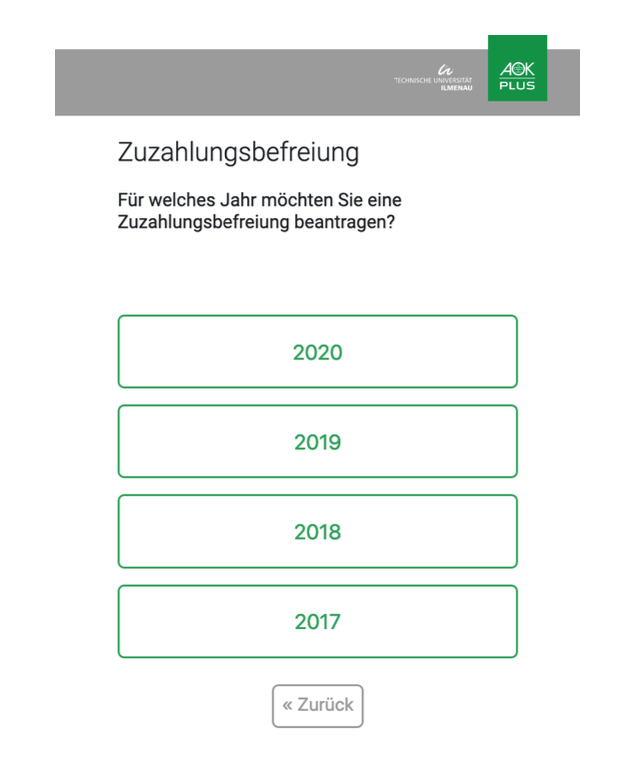
\includegraphics[width=10cm , height=12cm]{Bilder/Interface.png}
    \caption{Benedikt Bieberle, Niclas Deppisch und Robert Schwartz, "`Prototypische Entwicklung eines Self-Service-Terminals für Wartebereiche von Krankenkassenfilianen"', Medienprojekt TU Ilmenau, Mai 2020}
    \label{fig:Interface}
\end{figure}
 \newpage
  \section{Nichtfunktionale Anforderungen}
\vspace{1cm}

\begin{itemize}
    \item \textbf{/N010/} \textit{Intuitive Bedienbarkeit:} \par
    Die Benutzeroberfläche muss übersichtlich gestaltet werden. Dafür empfehlen sich bildschirmfüllende Schaltflächen mit kontrastreichen Farben. Es sollen nach Möglichkeit nicht mehr als fünf Schaltflächen pro Seite angezeigt werden. 
    
    \item \textbf{/N020/} \textit{Nur eindeutige Eingaben möglich:} \par
    Ein Nutzer soll nur Eingaben tätigen können, die eindeutig sind und genau das ausführen, was sie suggerieren.
    
    \item \textbf{/N030/} \textit{Hohe Performanz:} \par
    Die Reaktionszeit der Benutzeroberfläche beim Klick auf eine Schaltfläche soll dauerhaft unter einer Sekunde liegen.
    
    \item \textbf{/N040/} \textit{Zuverlässigkeit:} \par
    Es soll ein Dauerbetrieb möglich sein. Bei einem Ausfall von Clients soll das System sich automatisch neustarten und wieder lauffähig sein.
    
    \item \textbf{/N050/} \textit{Wartungsarmer Betrieb:} \par
    Einmal eingerichtet soll das System möglichst keine Administratoreingriffe benötigen, bis auf das Aktuellhalten der Formulare und Einstellungen. Updates sollen nur in einem Zeitraum $> 3$ Monate nötig sein.
\end{itemize}{} \newpage
  \section{Qualitätszielbestimmungen}

%\comment{Auf welche Qualitätsanforderungen (Zuverlässigkeit, Robustheit, Benutzungsfreundlichkeit, Effizienz, ...) wird besonderen Wert gelegt?}

\begin{center}
 \begin{tabular}{l|c|c|c|c}
  ~ & sehr wichtig & wichtig & weniger wichtig & unwichtig\\
  \hline \hline
  \textit{Robustheit}~ &  ~ ~ ~ & \textbf{X}~ &  ~ ~ ~ &  ~ ~ ~ \\
  \hline
  \textit{Zuverlässigkeit}~ & \textbf{X}~ &  ~ ~ ~ &  ~ ~ ~ &  ~ ~ ~ \\
  \hline
  \textit{Korrektheit}~ &  ~ ~ ~ & \textbf{X}~ &  ~ ~ ~ &  ~ ~ ~ \\
  \hline
  \textit{Benutzerfreundlichkeit}~ &  \textbf{X}~ & ~ ~ ~ & ~ ~ ~ &  ~ ~ ~ \\
  \hline
  \textit{Effizienz}~ &  ~ ~ ~ & \textbf{X}~ &  ~ ~ ~ &  ~ ~ ~ \\
  \hline
  \textit{Portierbarkeit}~ &  ~ ~ ~ &  ~ ~ ~ & \textbf{X}~ &  ~ ~ ~ \\
  \hline
  \textit{Kompatibilität}~ &  ~ ~ ~ &  ~ ~ ~ & ~ ~ ~ & \textbf{X}~  \\
 \end{tabular}
\end{center}
 \newpage
  \section{Glossar}

\begin{description}
  \item[Back-End]
    Nur für Administratoren zugängliche Seiten zur Systemverwaltung, d.h. Einpflegen, Speichern, Bearbeiten, Exportieren und Löschen von Formularen sowie das Einstellen von Farbschemata und Logos im Front-End.
 
  \item[Django]
    ist ein in Python geschriebenes, quelloffenes Webframework, das einem Model-Template-View-Schema folgt.
    \footnote{\href{https://docs.djangoproject.com/en/dev/faq/general}{docs.djangoproject.com/en/dev/faq/general, abgerufen am 08.05.2020}}

   \item[Elektronische Gesundheitskarte]
    Chipkarte im Scheckkartenformat, die als erweiterte Versichertenkarte für gesetzlich Krankenversicherte fungiert.
    \footnote{\href{https://de.wikipedia.org/w/index.php?title=Elektronische_Gesundheitskarte&oldid=198562236}{de.wikipedia.org/w/index.php?title=Elektronische\_Gesundheitskarte,  abgerufen am 08.05.2020}}
    \footnote{\href{https://www.gesetze-im-internet.de/sgb_5/__291.html}{www.gesetze-im-internet.de/sgb\_5/\_\_291.html, abgerufen am 08.05.2020}}
 
  \item[Front-End]
    Webseite für die Kundenoberfläche.

  \item[iPad]
    Tabletcomputer des Herstellers Apple Inc.

  \item[Model Layer]
    Eine Abstraktionsschicht in Django, die zur Strukturierung und Manipulation von den Daten der Webapplikation dient.
    \footnote{\href{https://docs.djangoproject.com/en/3.0/}{docs.djangoproject.com/en/3.0/, abgerufen am 08.05.2020}}
 
  \item[Model-Template-View]
    Djangos Umsetzung des Model-View-Controller Musters.

  \item[Model-View-Controller]
    Model View Controller ist ein Muster zur Unterteilung einer Software in die drei Komponenten: Datenmodell (model), Präsentation (view) und Programmsteuerung (controller).
    \footnote{\href{https://de.wikipedia.org/w/index.php?title=Model_View_Controller&oldid=195305891}{de.wikipedia.org/w/index.php?title=Model\_View\_Controller, abgerufen am 08.05.2020}}
    
    \item[Python]
    ist eine universelle, interpretierte, multiparadigmatische Programmiersprache.
 
  \item[Views]
    in Django kapseln sie die Logik, welche für die Verarbeitung der Anfrage eines Nutzer und die Rückgabe einer Antwort verantwortlich ist.

  \item[Raspbian]
    Linux-Betriebssystem auf Basis von Debian. Wird hauptsächlich auf den Raspberry Pi Einplatinencomputern eingesetzt.

  \item[Self-Service-Terminal]
    Ein Computer, der von Kunden in einem Geschäft oder einer anderen Einrichtung zur Selbstbedienung genutzt werden kann. Oftmals mit eingebautem Touchscreen.
\end{description}

\end{document}
